\appendix
\section{Cluster-Permutation PSD Anchor Tests (Supplementary)}
\label{app:psd_anchor}

To triangulate contrast strength with FM-independent empirical
evidence, we ran the same cluster-permutation PSD protocol on three
datasets: UCSD Stress (the primary cohort under audit), EEGMAT (the
anchored arm of the paired experiment), and TDBRAIN (the
intermediate-anchor case study). The protocol is identical across
datasets to enable apples-to-apples comparison; only cohort sizes,
channel counts, and label axes differ.

\paragraph{Protocol.} For each recording, Welch power spectral
density estimates were computed from the cached 5\,s epochs
(2\,s Hamming windows, 50\% overlap, $0.5$--$45$\,Hz at $\Delta f =
0.5$\,Hz), averaged across non-overlapping epochs and
log-transformed to a $(N_\text{rec}) \times (C) \times (F = 90)$
tensor. MNE \texttt{permutation\_cluster\_test} (two-tailed) was run
with 1000 permutations at the default $F$-threshold corresponding to
$p = 0.05$ and independent adjacency across channels and frequency
bins. The two groups compared per dataset are the two classes of the
primary downstream label.

\subsection*{A.1 --- UCSD Stress (Bounded)}
\label{app:psd_stress}
Cohort: $70$ recordings, DASS-high ($n = 14$) vs DASS-low ($n = 56$),
$30$ channels. \emph{No cluster survived the pre-registered
$p < 0.05$ threshold.} Five candidate clusters emerged; minimum
cluster-corrected $p = 0.096$. The largest subthreshold cluster
spanned theta--alpha ($4$--$12$\,Hz) over 17 fronto-central
electrodes with within-cluster Hedges' $g = +0.82$ (DASS-high $>$
DASS-low). Whole-scalp band-averaged effect sizes were theta
$g = +0.57$, alpha $g = +0.59$, $|g| \leq 0.13$ elsewhere
(Fig.~\ref{fig:stress_psd_anchor}).

\begin{figure}[!t]
\centering
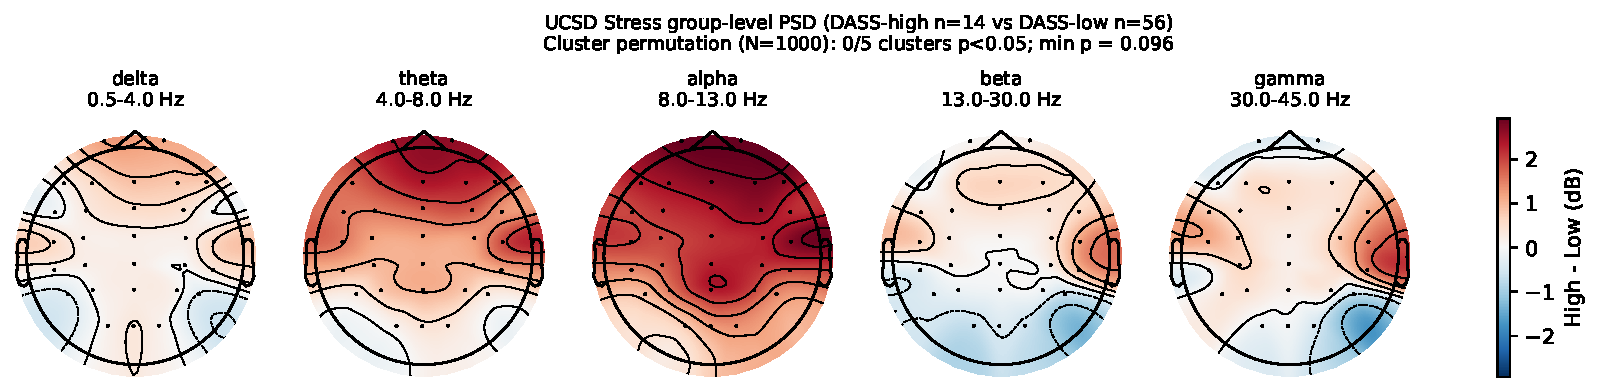
\includegraphics[width=0.95\linewidth]{figures/supplementary/fig_stress_psd_anchor.pdf}
\caption{UCSD Stress pre-registered cluster-permutation PSD
  ($14$ vs $56$). No cluster survived $p < 0.05$ cluster-corrected;
  subthreshold theta--alpha cluster is directionally consistent with
  arousal literature but does not meet the anchor criterion.}
\label{fig:stress_psd_anchor}
\end{figure}

\subsection*{A.2 --- EEGMAT (Strong-anchored)}
\label{app:psd_eegmat}
Cohort: $72$ recordings, task ($n = 36$) vs rest ($n = 36$), $19$
channels. \emph{One cluster survived correction at $p = 0.048$},
spanning $6$--$11.5$\,Hz over $17$ channels with within-cluster
Hedges' $g = -0.79$ (task $<$ rest), localised to the theta--alpha
band with posterior emphasis. Whole-scalp band-averaged effect sizes
were alpha $g = -0.66$, theta $g = -0.26$, gamma $g = +0.36$, $|g|
\leq 0.25$ elsewhere. The cluster's spectral locus and sign (alpha
desynchronisation during cognitive load) are textbook Klimesch-type
alpha-ERD \citep{klimesch1999,pfurtscheller1979}
(Fig.~\ref{fig:eegmat_psd_anchor}).

\begin{figure}[!t]
\centering
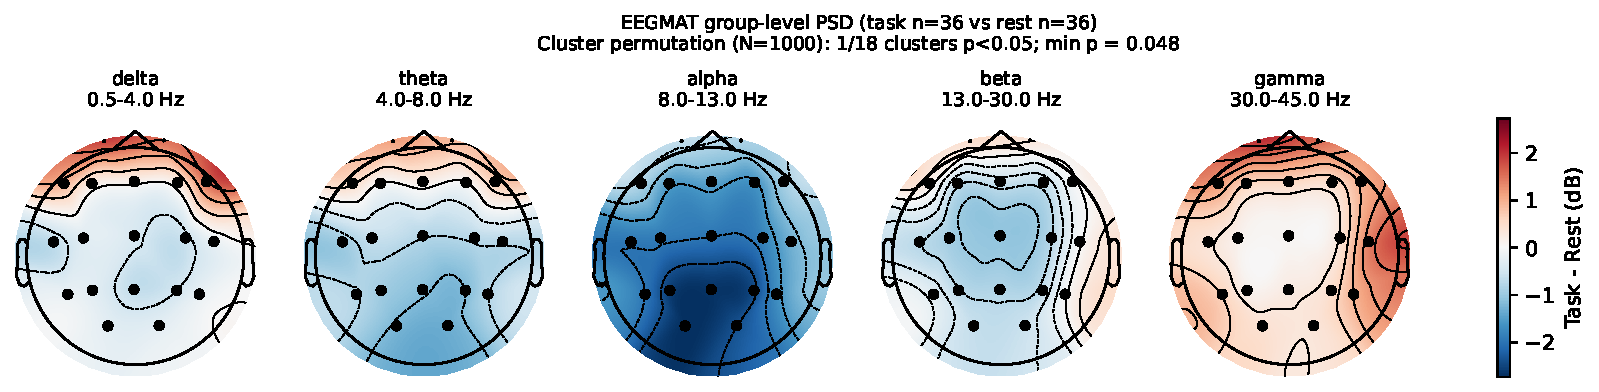
\includegraphics[width=0.95\linewidth]{figures/supplementary/fig_eegmat_psd_anchor.pdf}
\caption{EEGMAT cluster-permutation PSD ($36$ task vs $36$ rest).
  One cluster at $p = 0.048$ over $17$ posterior channels
  spanning $6$--$11.5$\,Hz with $g = -0.79$, consistent with
  Klimesch alpha-ERD. Literature + cluster + locus agree;
  Strong-anchored.}
\label{fig:eegmat_psd_anchor}
\end{figure}

\subsection*{A.3 --- TDBRAIN (Intermediate)}
\label{app:psd_tdbrain}
Cohort: $734$ recordings (EO + EC), MDD ($n = 640$) vs HC
($n = 94$), $19$ channels. \emph{Two clusters survived correction}:
cluster A at $p = 0.012$, $12.5$--$45$\,Hz over $8$ channels with
within-cluster $g = +0.42$; cluster B at $p = 0.014$,
$21.5$--$45$\,Hz over $7$ channels with $g = +0.40$. Whole-scalp
band-averaged effect sizes were beta $g = +0.35$, gamma $g = +0.33$,
alpha $g = -0.16$, $|g| \leq 0.23$ elsewhere
(Fig.~\ref{fig:tdbrain_psd_anchor}).

The empirical cluster survives correction but occupies the
beta/gamma band, not the alpha asymmetry locus predicted by the
published MDD-EEG literature the classification was originally
motivated by. A beta/gamma elevation is directionally consistent
with cortical hyperarousal literature in depression
\citep{olbrich2013mddarousal} but has not been established as a
per-recording within-subject correlate. Under the three-dimension
rubric of Sec.~\ref{sec:methods_anchor} this discordance between
empirical cluster locus and published within-subject locus classifies
TDBRAIN as \emph{Intermediate}. We note the large cohort imbalance
($640$ vs $94$) as a power caveat that amplifies small effects and
urge caution in reading the cluster-$p$ as a direct anchor-strength
proxy; the locus-concordance dimension is the load-bearing
classifier.

\begin{figure}[!t]
\centering
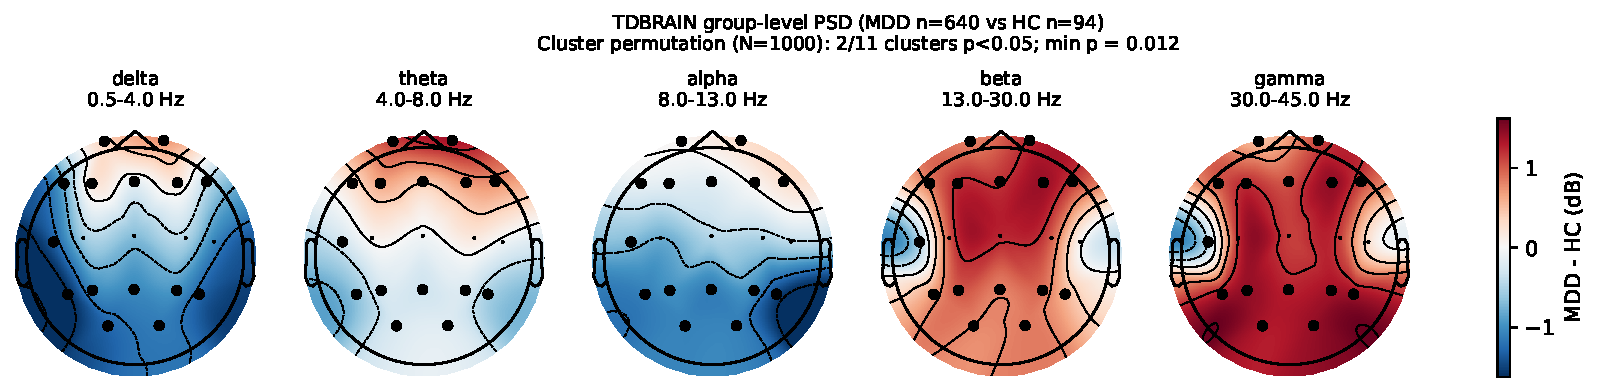
\includegraphics[width=0.95\linewidth]{figures/supplementary/fig_tdbrain_psd_anchor.pdf}
\caption{TDBRAIN MDD vs HC cluster-permutation PSD ($640$ vs $94$).
  Two clusters survive correction (min $p = 0.012$) but localise to
  beta/gamma, not the published alpha-asymmetry locus. Empirical
  effect exists but does not align with the literature-anchored
  within-subject correlate; Intermediate-anchored.}
\label{fig:tdbrain_psd_anchor}
\end{figure}

\paragraph{Cross-dataset summary.} The three datasets span the
operating range of our three-dimension rubric:

\begin{table}[!htbp]
\centering
\small
\caption{Empirical cluster-permutation anchor summary.}
\label{tab:anchor_matrix}
\begin{tabular}{lccc}
\toprule
Dataset      & Published w.-s. correlate & Cluster at $p < 0.05$ & Locus match \\
\midrule
EEGMAT       & yes (Klimesch $\alpha$-ERD)   & yes ($p = 0.048$) & yes (alpha-ERD)   \\
TDBRAIN MDD  & no (cross-subj. only)         & yes ($p = 0.012$) & no (beta/gamma)   \\
UCSD Stress  & no                            & no ($p = 0.096$)  & ---               \\
\bottomrule
\end{tabular}
\end{table}

\paragraph{Interpretation.} The three rows correspond directly to
the three regimes on the Fig.~\ref{fig:sdl_spectrum} SDL spectrum:
Strong-anchored (EEGMAT, all three dimensions agree),
Intermediate-anchored (TDBRAIN, empirical cluster without literature
or locus support), and Bounded (UCSD Stress, no surviving cluster
and no published correlate). The behavioural FM rescue pattern
(EEGMAT rescues uniformly across three FMs; TDBRAIN produces a
$19$\,pp architecture spread; UCSD Stress bounded at
$0.52$--$0.58$) tracks this empirical ordering without being
conditioned on FM outputs.
